\chapter{Supersymmetry and the MSSM}\label{ch:supersymmetry}

Historically, examining nature at increasing energy scales (and correspondingly decreasing length scales ) has consistently yielded new physics. For example, higher-energy experiments were able to probe the structure of the weak interactions, precisely at the energy scale that the 4-Fermi theory started to fail. Similarly, the challenges listed at the end of \autoref{ch:sm} most likely point to new physics at higher energy scales, between the currently explored weak scale to the reduced Planck scale:
\begin{equation*}
M_P = 1/\sqrt{8\pi G} \approx 2.4\times 10^{18} \text{ GeV}
\end{equation*}
However, the SM Higgs potential is extremely sensitive to new physics at high energies. The mass of the SM Higgs boson receives large quantum corrections from any new physics at high energies that couples to the Higgs sector. For example, if the Higgs couples to a heavy fermion \emph{f} through a term of the form $-\lambda_fH\bar{f}f$, the one-loop correction to the higgs mass takes the form
\begin{equation}
\Delta m_H^2 = -\frac{|\lambda_f|^2}{8\pi^2}\Lambda_\text{UV}^2 + ...
\label{eq:one_loop_fermion}
\end{equation}
where $\Lambda_{UV}$ is some cutoff momentum where the effects of the new physics are expected to manifest themselves. Similarly, the one-loop correction from a heavy scalar \emph{S} through the term $-\lambda_S|H|^2|S|^2$ takes the form
\begin{equation}
  \Delta m_H^2 = \frac{\lambda_S}{16\pi^2}\left[\Lambda_\text{UV}^2 + ...\right]
\label{eq:one_loop_scalar}
\end{equation}
In both these cases, the size of the correction scales quadratically with the momentum cutoff $\Lambda_{UV}$. Higher-order loop corrections can be shown to be similarly large as well. Thus the `natural' mass of the Higgs would seem to be on the the order of $\Lambda_{UV}$, which could even be as high as the Planck scale. In contrast, the actual mass that we measure is only about 126 GeV. Thus there is a \emph{hierarchy} between the observed and the `natural' mass of the SM Higgs, one of many orders of magnitude. \footnote{Note that even though only the mass of the SM Higgs is directly sensitive to $\Lambda_{UV}$, this sensitivity is propagated to all the other SM particles through their couplings to the SM Higgs.}
Thus it would seem that any UV completion of the SM would have to come with a host of parameters to tune the counterterms enough to cancel out the quadratic divergences and result in the physical mass we observe experimentally. If the new physics is at the Planck scale, the divergences must cancel to less than one part in $10^{-16}$ to give us a SM Higgs at the weak scale.
It is obviously undesirable to have to manually tune a large number of parameters to be able to come up with UV completions of the Standard Model - it would be analogous to the geocentric Ptolemaians adding an ever-increasing number of epicycles to explain what would ultimately be more simply and accurately described by Copernicus's heliocentric theory. 
Looking at the forms of the one-loop corrections in \autoref{eq:one_loop_fermion} and \autoref{eq:one_loop_scalar}, we can see that the contribution from the fermion \emph{f} will be exactly canceled out by the contributions from two complex scalars \footnote{Thus matching the number of fermionic and scalar degrees of freedom.} with $\lambda_S = |\lambda_f|^2$, the corrections from the scalar and the fermion will cancel out exactly. This suggests that the simplest way to ensure that all quadratic divergences from new physics at high energy scales cancel out is to require some kind of symmetry between fermions and scalars, ensuring that there is a scalar partner for each fermion, or vice versa.

This symmetry is known as \emph{supersymmetry}. It is a rich mathematical structure with far-reaching consequences, a lot of which are beyond the scope of this work. For a pedagogical review of supersymmetry, we refer the reader to \citep{Martin1997}. This section provides a necessarily condensed version of the treatment there. Although the hierarchy problem has been the main driving force behind the development of supersymmetry, there are other benefits that can be obtained, such as gauge coupling unification and a stable dark matter candidate, that we shall revisit in future sections.

The term `supersymmetry' refers to the invariance of the Lagrangian under supersymmetry transformations of the form
\begin{align*}
  Q|\text{Boson}\rangle = |\text{Fermion}\rangle &&\text{and}&& Q|\text{Fermion}\rangle = |\text{Boson}\rangle.
\end{align*}

\section{Construction of supersymmetric Lagrangians}
In this section, we will briefly describe how to construct the Lagrangian of a general supersymmetric theory, using the superfield formalism. We will follow the approach in \citep{Zee2010}, which in turn is an exposition of the procedure in \citep{Salam1974}.

\section{Stable dark matter candidate}
The MSSM has a new kind of symmetry known as \emph{R-parity}. It is an analogue of baryon and lepton number conservation. The Lagrangian of the MSSM is defined to be invariant under the action of the operator $P_R$ on the fields. The eigenvalues of this operator are $(-1)^{3(B-L)+2s}$, where \emph{B, L}, and \emph{s} represent the baryon number, lepton number, and spin of the particle, respectively. The  

The consequence of this is that the lightest supersymmetric particle (LSP) must be absolutely stable, that is, it cannot decay further into other particles.

\section{Gauge coupling unification}
Another motivation for the MSSM is that it has the right particle content to unify the strong and electroweak couplings at a high energy scale, as seen in \autoref{fig:gauge_coupling_unification}.

\begin{marginfigure}
    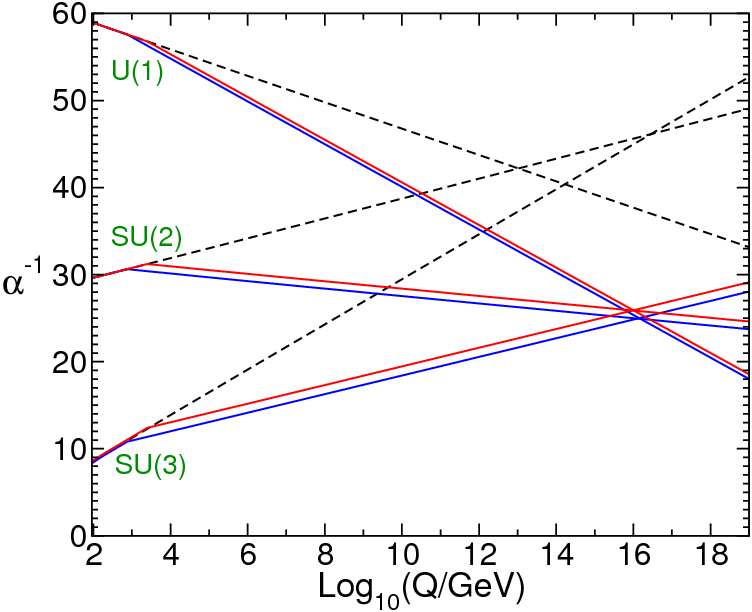
\includegraphics[width=\textwidth]{images/gauge_coupling_unification}
  \caption{2-loop RG evolution of inverse gauge couplings in the SM (dashed lines) and the MSSM (solid lines). The sparticle masses are varied between 0.5-1.5 TeV, and $\alpha_3(m_Z)$ is varied between 0.117 and 0.121. Source: \citep{Martin1997}.}
  \label{fig:gauge_coupling_unification}
\end{marginfigure}

\begin{marginfigure}
\feynmandiagram [layered layout, horizontal=b to c] { 
  a [particle=\(h\)] -- [scalar] b -- [fermion, half left, edge label=\(f\)] c -- [fermion, half left] b, c -- [scalar] d,
};
\begin{tikzpicture}
\begin{feynman}
  \vertex (a){\(h\)};
	\vertex [right=of a] (b);
	\vertex [right=of b] (c);
    \vertex [above=of b] (d);
\diagram*{
	{
      [edges = scalar]
      (a) -- (b) -- (c),
      (b) -- [half left, edge label=\(S\)] (d) -- [half left] (b),
    },
};
\end{feynman}
\end{tikzpicture}
\caption{One-loop corrections from fermions and scalars to the Higgs mass.}
\end{marginfigure}

\section{Supersymmetry basics}
\section{Chiral and gauge supermultiplets}
All the particles in the MSSM are grouped into structures known as supermultiplets. They come in two varieties: \emph{chiral} and \emph{gauge} supermultiplets. The SM fermions and the components of the SM Higgs doublet reside inchiral supermultiplets, and the SM gauge bosons reside in gauge supermultiplets. Let us first look at what the gauge interactions of a generic chiral and gauge supermultiplet look like.
For a generic chiral supermultiplet consisting of a complex scalar $\phi$ and its superpartner, a two-component Weyl fermion $\psi$, the kinetic terms are 
\[\mathcal{L}_{\text{chiral,kinetic,fermion}} = -\partial^\mu\phi^*\partial_\mu\phi + i\psi^{\dagger}\overline{\sigma}^\mu\partial_\mu\psi.\]
If the Lagrangian density is invariant under gauge transformations of the chiral supermultiplet under a gauge group with generators $(T^a)_i^j$ and associated gauge fields $A_\mu^a$, the partial derivatives above can be promoted to covariant derivatives:
\begin{align}
  \nabla_\mu\phi_i &= \partial_\mu\phi_i - igA_\mu^a(T^a\phi)_i\label{eq:phi1}\\
  \nabla_\mu\phi^{*i} &= \partial_\mu\phi^{*i} + igA_\mu^a(\phi^*T^a)^{i}\label{eq:phi2}\\
  \nabla_\mu\psi_i &= \partial_\mu\psi_i - igA_\mu^a(T^a\psi)_i\label{eq:psi}
\end{align}

\subsection{Interactions}
\subsection{The superpotential}
The MSSM superpotential takes the form
\[W_\text{MSSM} = \bar{u}\mathbf{y_u}QH_u-\bar{d}\mathbf{y_d}Q H_d-\bar{e}\mathbf{y_e}L H_d+\mu H_u H_d \]
\section{The MSSM superpotential}
\section{Split Supersymmetry}

The non-SM interactions in our signal process are the higgsino-bino-$Z$ and the higgsino-bino-$h$ interactions. To determine their coupling, we can inspect the structure of the MSSM. We will first examine the gauge interactions of higgsino and bino gauge eigenstates. Upon doing this, it will be apparent that there are no interaction terms containing both pure higgsinos and pure binos. The reason is that electroweak symmetry breaking induces mixing among the neutralinos. After this, we will move on to the coupling involving the SM Higgs boson, and see how it is obtained. 
In the MSSM, there are two $SU(2)_L\times U(1)_Y$ Higgs doublets instead of the one that we encounter in the standard model.
\[H_u = \begin{pmatrix}H_u^+\\H_u^0\end{pmatrix};
H_d = \begin{pmatrix}H_d^0\\H_d^-\end{pmatrix}\]
Inserting the covariant derivatives into the kinetic terms will yield the interaction terms. Each of the fields $H_u$ and $H_d$ can be interpreted as the scalar field $\phi$ in \autoref{eq:phi1} and \autoref{eq:phi2}. Similarly, the supersymmetrizations of $H_u$ and $H_d$,
\[\widetilde{H_u} = \begin{pmatrix}\widetilde{H_u}^+\\\widetilde{H_u}^0\end{pmatrix};
\widetilde{H_d} = \begin{pmatrix}\widetilde{H_d}^0\\\widetilde{H_d}^-\end{pmatrix}\]
can be equated with the field $\psi$ in \autoref{eq:psi}. The component fields of these are called \emph{higgsinos}. Once we insert the generators and associated gauge fields for the $SU(2)_L\times U(1)_Y$ symmetry in the covariant derivatives, and mix the gauge fields in the manner dictated by electroweak symmetry breaking, the gauge interactions of the higgs and higgsino fields look a lot like the SM interactions. In fact, they will have the same strength. Since we are interested in neutral higgsino-like NLSPs for our signal process, let us isolate their particular interaction terms:
\[\frac{g}{\cos\theta_W}Z_\mu\left(\widetilde{H_u}^{0\dagger}\overline{\sigma}^\mu \widetilde{H_u}+
\widetilde{H_d}^{0\dagger}\overline{\sigma}^\mu \widetilde{H_d}\right)\]
Now let us turn to the interactions of gauge supermultiplets. A generic gauge supermultiplet will consist of a gauge boson $A_\mu^a$ and its two-component Weyl fermion superpartner, the \emph{gaugino} $\lambda^a$. The SM gauge bosons reside in such gauge supermultiplets, and so the index $a$ runs over the adjoint representation of the relevant gauge group. The gauge interactions of gauginos can be extracted from their kinetic term in the Lagrangian:
\[\mathcal{L}_{\text{gaugino,kinetic}} = i\lambda^{a\dagger}\overline{\sigma}^\mu\nabla_\mu\lambda^a\]
where the covariant derivative is given by
\[\nabla_\mu\lambda^a = \partial_\mu\lambda^a + gf^{abc}A_\mu^b\lambda^c.\]
The factors $f^{abc}$ represent the structure constants of the gauge group. Thus, the interaction term would look like:
\[ig\lambda^{a\dagger}\overline{\sigma}^\mu f^{abc}A_\mu^b\lambda^c\]
The bino $(\widetilde{B}^0)$ is the superpartner of the SM gauge boson associated with the $U(1)_Y$ (hypercharge) gauge symmetry. Thus, it will transform in the adjoint representation of $U(1)_Y$ as well. However, this implies that there can never be a interaction vertex containing a bino and a gauge boson, since the structure constants for $U(1)_Y$ are all simply 0. In addition, we have previously seen that examining the chiral supermultiplet conaining the higgsino does not yield a neutral higgsino-bino-$Z$ vertex either. The reason that we can consider such a vertex in our signal process is due to the fact that electroweak symmetry breaking induces mixing among neutral higgsinos, binos, and the neutral wino $(\widetilde{W}^0)$, the superpartner of the $W_\mu^3$ gauge field associated with the SM $SU(2)_L$ gauge symmetry that mixes with $B_\mu$ to form the $Z$ boson and photon.

